%%%%%%%%%%%%%%%%%%%%%%%%%%%%%%%%%%%%%%%%%
% Thin Sectioned Essay
% LaTeX Template
% Version 1.0 (3/8/13)
%
% This template has been downloaded from:
% http://www.LaTeXTemplates.com
%
% Original Author:
% Nicolas Diaz (nsdiaz@uc.cl) with extensive modifications by:
% Vel (vel@latextemplates.com)
%
% License:
% CC BY-NC-SA 3.0 (http://creativecommons.org/licenses/by-nc-sa/3.0/)
%
%%%%%%%%%%%%%%%%%%%%%%%%%%%%%%%%%%%%%%%%%

%----------------------------------------------------------------------------------------
%	PACKAGES AND OTHER DOCUMENT CONFIGURATIONS
%----------------------------------------------------------------------------------------

\documentclass[a4paper, 11pt]{article} % Font size (can be 10pt, 11pt or 12pt) and paper size (remove a4paper for US letter paper)

\usepackage[protrusion=true,expansion=true]{microtype} % Better typography
\usepackage{graphicx} % Required for including pictures
\usepackage{wrapfig} % Allows in-line images

\usepackage{mathpazo} % Use the Palatino font
\usepackage[T1]{fontenc} % Required for accented characters
\linespread{1.05} % Change line spacing here, Palatino benefits from a slight increase by default

\makeatletter
\renewcommand\@biblabel[1]{\textbf{#1.}} % Change the square brackets for each bibliography item from '[1]' to '1.'
\renewcommand{\@listI}{\itemsep=0pt} % Reduce the space between items in the itemize and enumerate environments and the bibliography

\renewcommand{\maketitle}{ % Customize the title - do not edit title and author name here, see the TITLE block below
\begin{flushright} % Right align
{\LARGE\@title} % Increase the font size of the title

\vspace{50pt} % Some vertical space between the title and author name

{\large\@author} % Author name
\\\@date % Date

\vspace{40pt} % Some vertical space between the author block and abstract
\end{flushright}
}

%----------------------------------------------------------------------------------------
%	TITLE
%----------------------------------------------------------------------------------------

\title{\textbf{Exploiting LED Rolling-Shutter Effect in Indoor Positioning System}\\ % Title
Modern Mobile Communications} % Subtitle

\author{\textsc{Yang Guang} % Author
\\{\textit{1140339072}}} % Institution

\date{\today} % Date

%----------------------------------------------------------------------------------------

\begin{document}

\maketitle % Print the title section

%----------------------------------------------------------------------------------------
%	ABSTRACT AND KEYWORDS
%----------------------------------------------------------------------------------------

%\renewcommand{\abstractname}{Summary} % Uncomment to change the name of the abstract to something else

\begin{abstract}
It has been very mature to locate one's position in the outdoors using GPS like satellite positioning systems in a relatively acceptable deviation. However, Indoor Positioning System(IPS), still cannot be available in modern indoor environment such as airport or grand shopping plazas due to several constrains. But IPS has been proved to be very useful in the perspective future by the industry. Although this topic has been researched in recent 10 years in many related methods, there are two key issues of hardware cost against accuracy that cannot make a good balance between one another. In this article, we first give some research on related works of indoor positioning system, mainly on five systems of RADAR[00], Centaur[12], Cricket[04], Ubicarse[14], and Luxapose[14], then we fuifill the detail implementation of Luxapose, one method exploits visible light communication to realize IPS and evaluate its performance on some key factors of accuracy and available limit distance.
\end{abstract}

\hspace*{3,6mm}\textit{Keywords:} IPS , AoA , Rolling Shutter, VLC % Keywords

\vspace{30pt} % Some vertical space between the abstract and first section

%----------------------------------------------------------------------------------------
%	ESSAY BODY
%----------------------------------------------------------------------------------------

\section*{1. Introduction}

 Smart devices with cameras and LEDs are abundant in today's environment. This abundance creates an untapped opportunity for using these devices for wireless communication. Meanwhile, even if localization technology based on GPS developed maturely, we find the inconvenience with indoor localizations in malls or airports, which in fact in great need of the technology support of indoor localization since the environment is complex. Indoor localization serves these situations, and it can detect a wireless user's gesture, movement, or can do location-based authentication. In this article we draws a novel way by exploiting the LED lights to realize this indoor localization problem. 

 

This report does some survey on existing indoor localization methods and introduces some representative works in section 2. In section 3 we explicit the major task of Luxapose, involving the working scenario and techniques we planned to utilize, then we give a detailed definition of the indoor localization with LED AoA algorithm. In section 4 we introduced how the system been built on different modules. In section 5 we make an evaluation on several key metrics of location distance and accuracy and look forward to some future work that are needed to be worked on.

%------------------------------------------------

\section*{2. Related Works}
Indoor localization has been worked on for years since its demand in industry is badly. We review four major representative work based on RF, acoustic, and MIMO techniques, the four main methods today in research of indoor localization. We analysis their defects to show the advancement in our work of Indoor Localization with LEDs.

\subsection*{2.1 RF-based Localization \cite{Radar00} \cite{Centaur12}}
\subsubsection*{2.1.1 RF-based Localization \cite{Radar00} \cite{Centaur12}}
\subsubsection*{2.1.2 RF-based Localization \cite{Radar00} \cite{Centaur12}}

\subsection*{2.2 Acoustic-based Localization \cite{Cricket04}}

\subsection*{2.3 MIMO-based Localization \cite{Ubicarse14}}

Cras gravida, est vel interdum euismod, tortor mi lobortis mi, quis adipiscing elit lacus ut orci. Phasellus nec fringilla nisi, ut vestibulum neque. Aenean non risus eu nunc accumsan condimentum at sed ipsum.
\begin{wrapfigure}{l}{0.4\textwidth} % Inline image example
\begin{center}
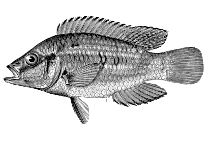
\includegraphics[width=0.38\textwidth]{fish.png}
\end{center}
\caption{Fish}
\end{wrapfigure}
Aliquam fringilla non diam sed varius. Suspendisse tellus felis, hendrerit non bibendum ut, adipiscing vitae diam. Lorem ipsum dolor sit amet, consectetur adipiscing elit. Nulla lobortis purus eget nisl scelerisque, commodo rhoncus lacus porta. Vestibulum vitae turpis tincidunt, varius dolor in, dictum lectus. Aenean ac ornare augue, ac facilisis purus. Sed leo lorem, molestie sit amet fermentum id, suscipit ut sem. Vestibulum orci arcu, vehicula sed tortor id, ornare dapibus lorem. Praesent aliquet iaculis lacus nec fermentum. Morbi eleifend blandit dolor, pharetra hendrerit neque ornare vel. Nulla ornare, nisl eget imperdiet ornare, libero enim interdum mi, ut lobortis quam velit bibendum nibh.

Morbi tempor congue porta. Proin semper, leo vitae faucibus dictum, metus mauris lacinia lorem, ac congue leo felis eu turpis. Sed nec nunc pellentesque, gravida eros at, porttitor ipsum. Praesent consequat urna a lacus lobortis ultrices eget ac metus. In tempus hendrerit rhoncus. Mauris dignissim turpis id sollicitudin lacinia. Praesent libero tellus, fringilla nec ullamcorper at, ultrices id nulla. Phasellus placerat a tellus a malesuada.

%------------------------------------------------

\section*{3. Problem Definition and Algorithm of Luxapose}

Fusce in nibh augue. Cum sociis natoque penatibus et magnis dis parturient montes, nascetur ridiculus mus. In dictum accumsan sapien, ut hendrerit nisi. Phasellus ut nulla mauris. Phasellus sagittis nec odio sed posuere. Vestibulum porttitor dolor quis suscipit bibendum. Mauris risus lectus, cursus vitae hendrerit posuere, congue ac est. Suspendisse commodo eu eros non cursus. Mauris ultrices venenatis dolor, sed aliquet odio tempor pellentesque. Duis ultricies, mauris id lobortis vulputate, tellus turpis eleifend elit, in gravida leo tortor ultricies est. Maecenas vitae ipsum at dui sodales condimentum a quis dui. Nam mi sapien, lobortis ac blandit eget, dignissim quis nunc.

\begin{enumerate}
\item First numbered list item
\item Second numbered list item
\end{enumerate}

Donec luctus tincidunt mauris, non ultrices ligula aliquam id. Sed varius, magna a faucibus congue, arcu tellus pellentesque nisl, vel laoreet magna eros et magna. Vivamus lobortis elit eu dignissim ultrices. Fusce erat nulla, ornare at dolor quis, rhoncus venenatis velit. Donec sed elit mi. Sed semper tellus a convallis viverra. Maecenas mi lorem, placerat sit amet sem quis, adipiscing tincidunt turpis. Cras a urna et tellus dictum eleifend. Fusce dignissim lectus risus, in bibendum tortor lacinia interdum.


\section*{4. System Modules Implementation}


\section*{5. Evaluation and Conclusion}

%----------------------------------------------------------------------------------------
%	BIBLIOGRAPHY
%----------------------------------------------------------------------------------------

\begin{thebibliography}{10}
	
\bibitem[Radar (2000)]{Radar00}
P.Bahl, V.N. Padmanabhan,
``Radar: An in-building RF-Based User Location and Tracking System.''
\textit{Proc. of IEEE INFOCOM}, volumn 2, pp. 775-784, 2000.

\bibitem[Cricket (2004)]{Cricket04}
Nissanka Bodhi Priyantha,
``The Cricket Indoor Location System.''
\textit{ACM SIGCOMM},2004.

\bibitem[Centaur (2012)]{Centaur12}
R.Nandakumar, K.K.Chintalapudi, and V.N.Padmanabhan,
``Centaur: Locating Devices in an Office Environment.''
\textit{ACM Mobicom},2012.

\bibitem[Luxapose (2014)]{Luxapose14}
Ye-Sheng Kuo, Pat Pannnuto,
``Luxapose: Indoor Positioning with Mobile Phones and Visible Light.''
\textit{ACM Mobicom},2014.

\bibitem[Ubicarse (2014)]{Ubicarse14}
Swarun Kumar, Stephanie Gil, Dina Katabi, Daniela Rus,
``Accurate Indoor Localization with Zero Start-up Cost.''
\textit{ACM Mobicom},2014.
\end{thebibliography}

%----------------------------------------------------------------------------------------

\end{document}